\documentclass[a4paper, oneside]{memoir}
\usepackage[utf8]{inputenc}
%\usepackage[T1]{fontenc}
\usepackage{verbatim}
\usepackage{graphicx}
\usepackage{listings}
\usepackage{listing}
\usepackage{amsthm}
\usepackage{amsfonts}
\usepackage{amsmath}
\usepackage{subfig}
\usepackage{varioref}
\usepackage{color}
\usepackage{pgf}
\usepackage[colorinlistoftodos]{todonotes}
%\usepackage[colorlinks, linkcolor=blue, citecolor=red, urlcolor=brown]{hyperref}
\usepackage{hyperref}
% ^- farver gør det meget nederen at udskrive en s/h kopi, da alle "se
% fig 1.1 på side xx" bliver grå! (ptx)

\usepackage{natbib}

%Individual todos
\newcommand{\todoPtx}[2][]{\todo[color=red,    #1]{Ptx: #2}}
\newcommand{\todoCpvc}[2][]{\todo[color=magenta, #1]{Cpvc: #2}}
\newcommand{\todoSean}[2][]{\todo[color=yellow,   #1]{Sean: #2}}
\newcommand{\todoHave}[2][]{\todo[color=green,  #1]{Have: #2}}
\newcommand{\todoVester}[2][]{\todo[color=blue,  #1]{Vester: #2}}

\renewcommand{\ttdefault}{pcr}


\lstset{language=C}
%\lstset{backgroundcolor=listinggray}
%\lstset{backgroundcolor=\color{listinggray}}
%\lstset{linewidth=90mm}
%\lstset{frameround=tttt}
%\lstset{frameround=trbl}
%\lstset{labelstep=1}
%\lstset{keywordstyle=\color{blue}\textbf}
\lstset{keywordstyle=\textbf}
%\lstset{moredelim=[is][\ttfamily]{|}{|}}
\lstset{basicstyle=\ttfamily \footnotesize}
%\lstset{basicstyle=\ttfamily \small}
%\lstset{commentstyle=\ttfamily}
\lstset{commentstyle=\normalfont \textit}
\lstset{stringstyle=\bfseries}
\lstset{showstringspaces=false}
%\lstset{numbers=left,numberstyle=\ttfamily \small}
%\lstset{breaklines=true}


% \lstset{
%   basicstyle=\ttfamily \footnotesize,
%   keywordstyle=\color{red}
% }


% Dokumantation:
% http://www.tex.ac.uk/tex-archive/macros/latex/contrib/todonotes/todonotes.pdf
% Vigtigste kommandoer:
% \todoVester[inline]{text}
% \missingfigure{A illustration of how peers are placed on the ring}
% \todo{Introduction to this section}
% \todo[inline]{Someone write this}

% replaces cite. Use \cit instead!
\newcommand{\cit}[1] {\cite{#1}}

% cite with page or section ref
\newcommand{\citbook}[2] {\citep[#2]{#1}}

% when defining a new term
\newcommand{\dit}[1] {\textit{#1}}

% \image{image, scale, caption, label}
\newcommand{\image}[4]{
  \begin{figure*}[!htb]
    \centering
    \includegraphics[scale=#2]{imgs/#1}
    \caption{#3}
    \label{#4}
  \end{figure*}}
% ^- Det her går aldrig godt, man har aldrig brug for at ændre flere
% ting end der er muligt med denne slags makroer. (ptx)

\title{Level Sets!!}
\author{
 \\
  Martin Have (20051456)\\
  \url{have@cs.au.dk}\\
  \\
  Peter Kristensen (20051866)\\
  \url{ptx@cs.au.dk}\\
  \\
  Mikkel Vester (20053229)\\
  \url{vester@cs.au.dk}\\
  \\
  Christian P. V. Christoffersen (20050879)\\
  \url{cpvc@cs.au.dk}\\
  \\
  Sean Geggie (20052203)\\
  \url{geggie@cs.au.dk}\\
  \\
  University of Aarhus
}

\begin{document}

\maketitle{}


\missingfigure{Her er et billede af et morph ting}

% Hvem laver hvad.
\begin{comment} % orgtbl-mode er win
|----------------------------+----------+--------|
| Afsnit                     | Indhold  | Hvem   |
|----------------------------+----------+--------|
| Intro                      | ch. 1,2  | have   |
| Build SDF / Discretization | artikel? | vester |
| Reinitialize               | ch. 7    | cpvc   |
| Motion                     | ch. 4,6  | ptx    |
| Externally gen. vf.        | ch. 3    | geggie |
| Godunov                    | ch. 5    | cpvc   |
|----------------------------+----------+--------|
\end{comment}

\newpage

\tableofcontents{}
\listoftodos
\chapter{Introduction}
\label{chap:introduction}
  In this report, we will explain what the Level Set method is and what
its applications are. Furthermore, we will provide code examples of
how to implement the mathematical formulas needed to create a Level
Set framework.

The Level Set method is a numerical technique used to transform
surfaces in $d$ dimensions. Transform means that we move the surface. The surfaces are transformed by solving a
partial differential equation(PDE) dependant on a time factor.

The level set at its most simple representation is a static
datastructure. It can be represented as a topographic map indicating
heights in a region, displayed in figure \vref{fig:isocontour-2d} or
it can be seen as a meteorological map, displaying weather data like
pressure. 
In figure \vref{fig:heightmap} we see two figures describing a 2-d and 3-d view of an island. Figure \vref{fig:isocontour-2d} describes an isocontour map of heights where the color indicates the height of each point. The brighter the color the higher the point. Figure \vref{fig:isocontour-3d} shows the corresponding 3d view.  

\begin{figure}[h]
\begin{center}
  \subfloat[2D view of an elevation isocontour map]{
    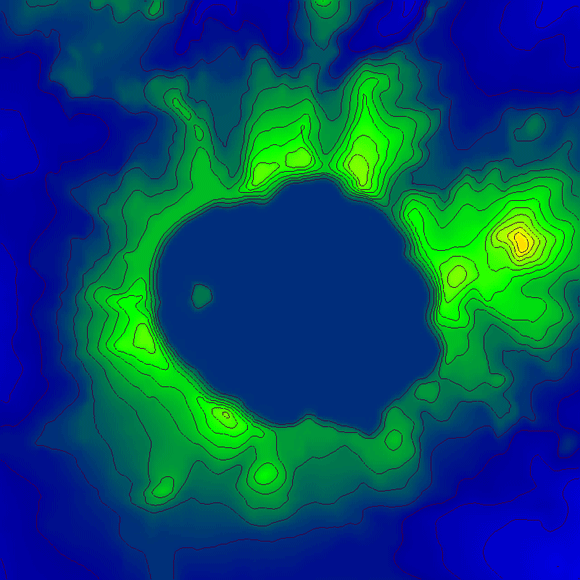
\includegraphics[width=0.5\textwidth]{imgs/226171_226171.png}
    \label{fig:isocontour-2d}
  }
  \subfloat[3D view of figure \ref{fig:isocontour-2d}]{
    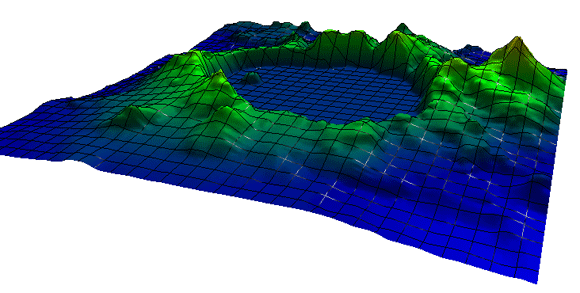
\includegraphics[width=0.5\textwidth]{imgs/226170_226170.png}
    \label{fig:isocontour-3d}
  }
\end{center}
\caption{Illustrations of heightmap, from: Intel Array Visualizer Gallery}
\label{fig:heightmap}
\end{figure}

%Intel Array Visualizer Gallery
%website\footnote{\url{http://www.intel.com/cd/software/products/apac/zho/perflib/226296.htm}}
\todoHave{husk reference}

%\image{hoejdekort.png}{0.25}{A topographic map indicating heights in the vermont region.}{introduction:fig:hoejdekort}

\section*{Signed distance function - $\phi$}

We would like a suitable way to indicate whether we are inside or outside the isocontour. 

We use an implicit representation of the surface. The Level Set method
can use implicit functions which means that the function is defined in
the entire plane and not only on the object.

The function $\phi(x,y)$ is a signed distance function in all of
$\mathbb{R}^{n}$, in our case $\mathbb{R}^{2}$. A signed distance
function $\phi$ is a function that given a point on the plane, returns
the distance to the surface. We have that $\phi(x,y) > 0$ if we are
outside the object and $\phi(x,y) < 0$ when we are inside the object.
And last, when $\phi(x,y) = 0$ we are on the interface or iso-surface.
The iso-surface separates the inside and outside.  Besides indicating
whether we are inside or outside an object, it also indicates how far
we are from the closest point on the iso-surface which is quite
handy. For a picture of the above, see figure
\vref{introduction:fig:implicitfunction}.

\image{phi.png}{0.3}{The figure is borrowed from
\cit{osher2002level}. A implicit function, defined in all of
$\mathbb{R}^{2}$. We see that when we are inside the object then
$\phi$ is less than zero, larger when we are outside and zero on the
interface.}{introduction:fig:implicitfunction}

%% Example - Circle

\subsection*{Example}

A simple example is to consider a circle and its equation:
\begin{equation*} 
  x^{2} + y^{2} = r^{2}
\end{equation*}

It is defined in all points in $\mathbb{R}^{2}$ and is an example of
an implicit function. Given a specific radius $r$, the equation of a
circle defines an isocontour. If $r = 5$, then the isovalue is $c =
5^{2} = 25$. For all the points $(x,y)$ that evaluate to 25 gives us
the isosurface. If the value is smaller then it is inside the surface,
and outside when the value is greater. See figure
\vref{introduction:fig:cartesiangrid}.


\section*{Cartesian grid}
\begin{comment} Finite memory -> descritization of plane -> cartesian
grid is used.
\end{comment}

Since a computer has finite memory we need to come up with a way to
store our representation. A simple way to do this that scale in the
number of dimensions is to partition the region into a grid where each
square is of equal size.

\begin{figure}[htb] \centering
    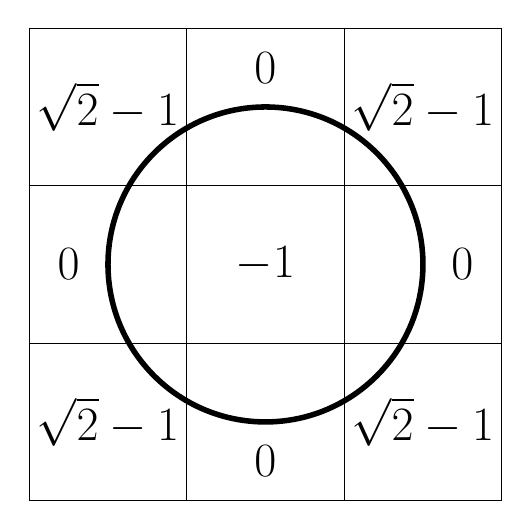
\begin{tikzpicture}[font=\LARGE]
    \draw (0,0) rectangle +(2,2)
    +(1,1) node {$-1$};
    \draw (0,2) rectangle +(2,2)
    +(1,1.5) node {$0$};
    \draw (2,0) rectangle +(2,2)
    +(1.5,1) node {$0$};
    \draw (0,-2) rectangle +(2,2)
    +(1,0.5) node {$0$};
    \draw (-2,0) rectangle +(2,2)
    +(0.5,1) node {$0$};
    \draw (2,2) rectangle +(2,2)
    +(1,1) node {$\sqrt{2}-1$};
    \draw (2,-2) rectangle +(2,2)
    +(1,1) node {$\sqrt{2}-1$};
    \draw (-2,2) rectangle +(2,2)
    +(1,1) node {$\sqrt{2}-1$};
    \draw (-2,-2) rectangle +(2,2)
    +(1,1) node {$\sqrt{2}-1$};
    \draw[line width=2pt] (1,1) circle (2);
  \end{tikzpicture}
  \caption{Borrowed from \cit{JLTGK}. A circle, descritized into a
cartesian grid. The value in each cell is the $\phi$ value described
in this chapter.}
  \label{introduction:fig:cartesiangrid}
\end{figure}

In figure \vref{introduction:fig:cartesiangrid}, we see how a plane
has been descritized into a cartesian grid, showing a circle and the
values of $\phi$.

%% formulas

\section*{Solving the Level Set}\label{sec:intro:solve} 

\todoPtx{I own this!!}

If we want to move the level set, we have to iteratively solve a Partial
differential equation to make the surface move. We solve a partial
differential equation in all points $(x,y) | x,y \in
\mathbb{R}^{2}$. If we want to move the interface in the normal
direction we solve the following equation:

\begin{equation}
\phi_{t} + a|\nabla \phi| = 0
\end{equation}\label{eq:normMove}

where $\nabla \phi = (\dfrac{\partial \phi}{\partial x},
\dfrac{\partial \phi}{\partial y})$ and $a$ can be of either sign.

When $a > 0$ the interface moves in the normal direction and when $a <
0$ it moves in the opposite direction of the normal.


\section*{Applications}

The advantages are that since we discretize the surface into a
cartesian grid, we can do numerical computations without having to
parameterize the objects. Another advantage is that the level set
method makes it easy to work on geometry that change topology over
time.


%% applications.  So why do we want to use the level set method? A
simple example is to consider an object that splits in two or two
objects merging into one. If we did not use the level set method, we
would have to explicitely represent the two new objects, where in the
level set case we get this for free do to the implicit representation.

\todoPtx{måske lidt flere anvendelsesmuligheder (lysberegninger her!)}

\newpage

\section*{Outline of the report}\todoPtx{Denne er på en side for sige
selv, så vref ikke crasher}

In chapter \vref{chap:sdf}, we give an in depth look on the signed
distance function, describe what kinds of mathematical operations we
have in our toolbox and describe the important reinitialize function,
section \vref{sec:reinitialize}.

In chapter \vref{chap:extensions}, we look at extension that can be
made to the basic level set implementation that we have done. In
section \vref{sec:segmentation}, we look at how to implement
segmentation algorithms which can be used in mediacal imaging. In
section \vref{sec:fluid}, we implement a fluid solver for computer
graphics using the level set method. And finally, in section
\vref{sec:imagereconstruction} \todoHave{Skal CPVC's afsnit være med i
den endelige rapport? (have)} we use the level set to do computations
on images.



%%% Local Variables: 
%%% mode: latex 
%%% mode: auto-fill 
%%% TeX-PDF-mode: t 
%%% TeX-master: "../master.tex" 
%%% End:



\chapter{SDF}
\label{chap:sdf}
\todoVester{tekst her}

\section{Mikkel-Sean Algorithm TM}
\label{sec:initialization}
\todo{Dette er et eksempel på en todo for alle}

\pagebreak
\section{Reinitialization}
\label{sec:reinitialize}
% -*- mode: latex; mode: auto-fill; coding: utf-8; -*-

The main advantage of representing an implicit counture or surface as
a signed distance field, is that the length of the gradient is
one. This is also exactly what defines a signed distance field.

When constructing or manipulating a signed distance field defined on a
Cartesean grid, the result is not always signed distance field. So to
enable further calculations or iterations of an algorithm the result
must be turned into a new signed distance field that reflexts the
changes done by the calculations. This process is called
\dit{reinitialization} of the level set, and can be done several
different ways.

Algorithms to reinitializing signed distance fields focuses on
reinitializing the whole domain, and at the same time keeping the zero
level set as fixed as possible. This means that the process disrupts
data outside the zero level set, which depending on the type of
phemomena we are modelling can be problematic. For the problems we are
modelling this is not an issue, and is therefore not of relevance here.

Before diving into the algoritms a good question is, how often must the
level set be reinitialized? There is no good answer to this question,
because it depends on how rapidly the contour is changing. In our work
we have been reinitializing after ever change, which ensures that this
is not a source of error.

The two most used algoritmic approched to reinitialization are:
geometricly methods that calculations distances to the contour or surface,
and PDE based methods that numerical approximates solutions to the Eikonal
equation: $||\nabla \phi|| = 1$ \citbook{book:fluids}{page~89}.

When initializing the implicit contour in section \vref{sec:initialization}
we used an algorithm that geometricly calculated the distance to the
contour. So the natural choise should be also to use this algorithm for
reinitializing, but because the algorithm does not calculate the
signed distance function precise enough, we cannot use this algorithm
when reinitializing. Furthermore if we had used this type of
algorithm, the we would have had to construct the contour before
invoking the algorithm. Constructing the contour is very expensive,
and is something that should be avoided at almost all cost when using
the level set method.

Instead we have chosen to use PDEs to solve the Eikonal
equation. Solving the Eikonal equation can also be done in different
ways, which we will describe in the next subsections.

\subsection{The PDE way of reinintalizing}
When using the PDE way of reinitialing the level set, we solve the
following PDE \citbook{book:levelset}{page~65-66}:

\begin{equation}
\label{eq:reinit}
\phi_t + S(\phi_0)(|\nabla \phi| - 1) = 0
\end{equation}

Where $\phi$ is the SDF being evolved as a PDE, and $\phi_0$, is the
initial SDF giving as input to the reinitialization algorithm, which
has not been altered by the process of solving the PDE. The function
$S(\phi_0)$ gives the sign of the SDF, like the following function,
described in \citbook{book:LS}{page~66}:
%\citbook{article:FLLSM}{page~419}:

\begin{equation}
\label{eq:s1}
S(\phi) =
\begin{cases}
-1 &\mbox{ if } \phi < 0, \\
 0 &\mbox{ if } \phi = 0, \\
 1 &\mbox{ if } \phi > 0.
\end{cases}
\end{equation}

When using this approach of reinitializing the SDF, then the grid
points in $\phi$ that are nearest to the contour is reinitialized
first, and then propergated in the normal direction from the zero
level set, hereby reinitializing the grids points in layers each
iteration.

This algorithm is relatively slow if all grid points needs to be
reinitialized, because it only reinitializes one layer in each
iteration when solving the PDE. This means that the PDE, on a
two-dimensional domain, must be iterated
$\sqrt{width^2 \times height^2}$ times to make sure that the algoritm
has reinitialized the whole domain.

But because the algorithm has the property of reinitializing the SDF
in layers it is of special interest in reguards to performance when
using a narrow band level set as described in section
\vref{sec:band}. Here only three or four layers around the SDF needs
to be reinitialized, making the algorithm ideal for the narrow band
approach.

\subsection{The sign function S}
Because equation \ref{eq:reinit} is a hyperbolic PDE, we need to use a
smeared out version of equation \eqref{eq:s1}. One way of smearing the
function is to using equation \eqref{eq:Sphi0}.

\begin{equation}
\label{eq:Sphi0}
S(\phi_0) = \frac{\phi_0}{\sqrt{\phi_0^2 + (\Delta x)^2}}
\end{equation}

The difference between equation \eqref{eq:s1} and equation
\eqref{eq:Sphi0}, can more easily be seen be looking at a plot of the
two functions, as depicted in figure \ref{fig:s-graph}.

\begin{figure}[h]
\begin{center}
  \subfloat[Plot of equation \eqref{eq:s1}]{
    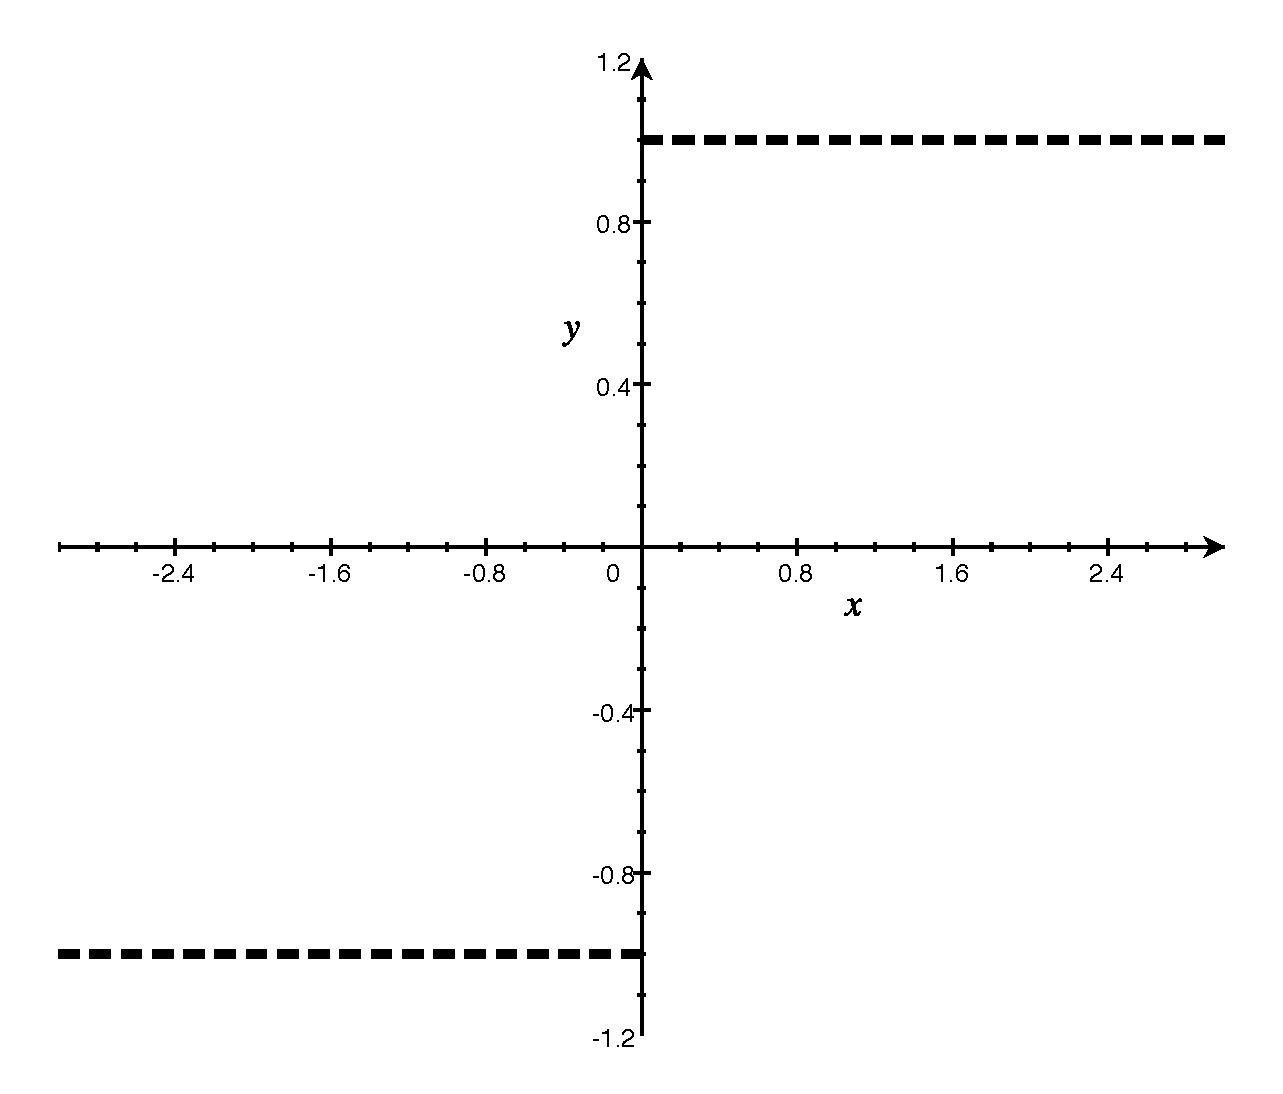
\includegraphics[width=0.5\textwidth]{imgs/S0.pdf}
    \label{fig:fake1}
  }
  \subfloat[Plot of equation \eqref{eq:Sphi0}, $\Delta x=1$]{
    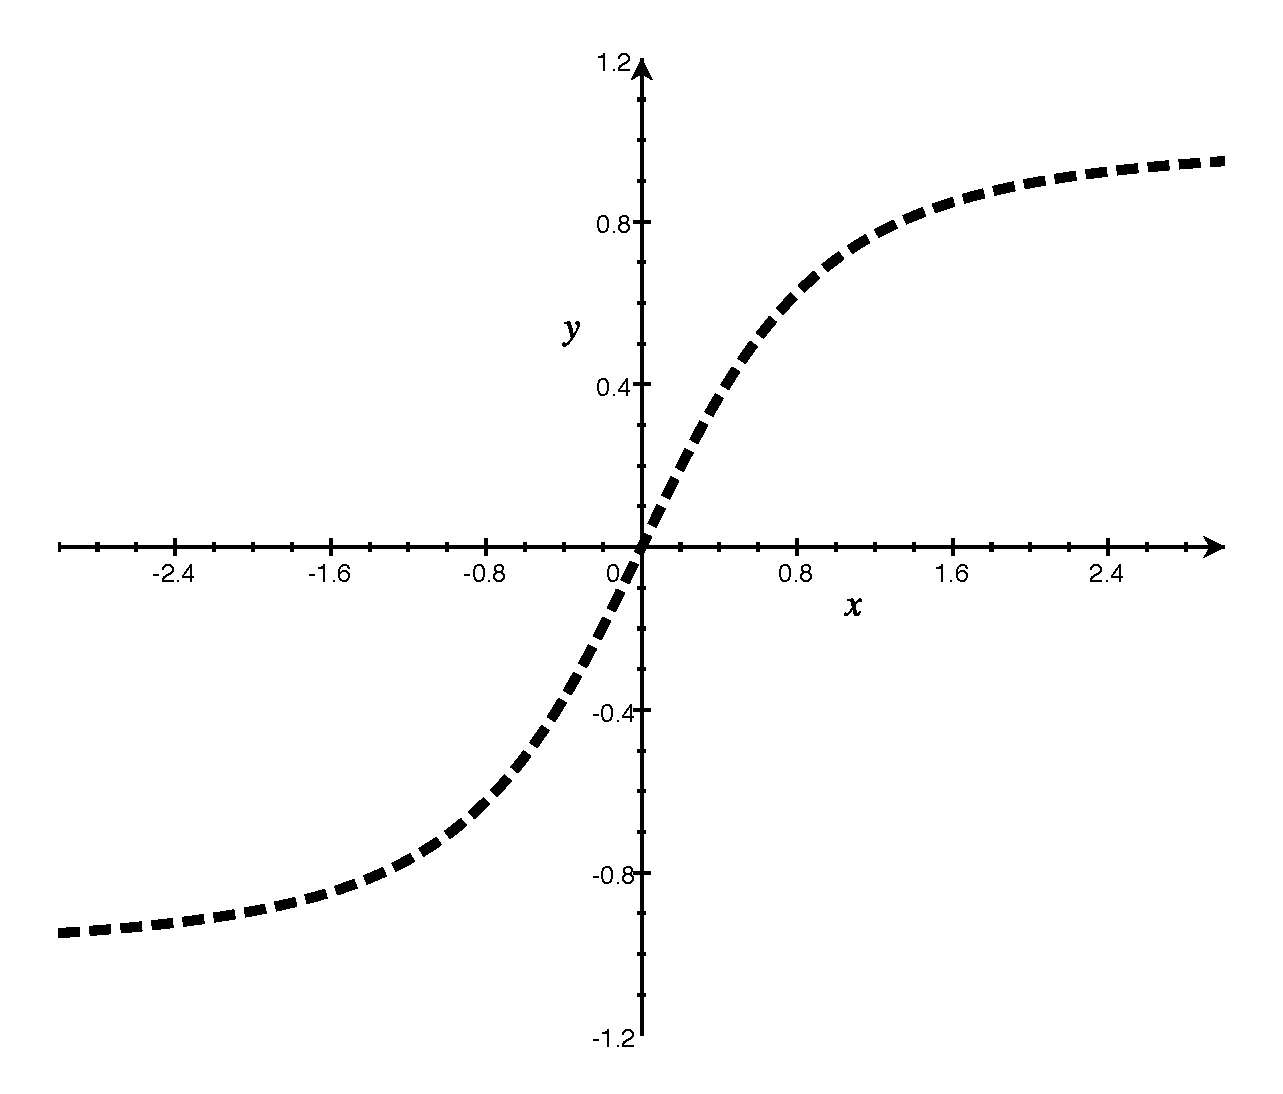
\includegraphics[width=0.5\textwidth]{imgs/S1.pdf}
    \label{fig:fake2}
  }
\end{center}
\caption{Illustrations of S}
\label{fig:s-graph}
\end{figure}

%\subsection{CFL-condition}


\pagebreak
\subsection{Implementation}
The implementation of how to solve the PDE from equation \eqref{},
uses the describtion Godunov's scheme from \citbook{book:LS}{page~58}
in the spatial dimensions, and a forward Euler in time, described in
formular (1.3) in \citbook{book:LS}{page~10}.

\begin{lstlisting}[language=c++]
    Tex<float> phi0 = GetPhi(); Tex<float> phin = GetPhi();
    for (unsigned int i = 0; i<iterations; i++) {
        for (unsigned int x = 0; x < width; x++) {
            for (unsigned int y = 0; y < height; y++) {
                float xy = phi(x, y);                
                float phiXPlus = 0.0f;
                float phiXMinus = 0.0f;
                float phiYPlus = 0.0f;
                float phiYMinus = 0.0f;        	
                if (x != width-1) phiXPlus  = (phi(x+1, y) - xy);
                if (x != 0)       phiXMinus = (xy - phi(x-1, y));
                if (y !=height-1) phiYPlus  = (phi(x, y+1) - xy);
                if (y != 0)       phiYMinus = (xy - phi(x, y-1));
        	
                float dXSquared = 0;
                float dYSquared = 0;
                float a = phi0(x,y);
                if (a > 0) {
                    // formula 6.3 page 58
                    float max = std::max(phiXMinus, 0.0f);
                    float min = std::min(phiXPlus, 0.0f);
                    dXSquared = std::max(max*max, min*min);
                    max = std::max(phiYMinus, 0.0f);
                    min = std::min(phiYPlus, 0.0f);
                    dYSquared = std::max(max*max, min*min);
                } else {
                    // formula 6.4 page 58
                    float max = std::max(phiXPlus, 0.0f);
                    float min = std::min(phiXMinus, 0.0f);
                    dXSquared = std::max(max*max, min*min);
                    max = std::max(phiYPlus, 0.0f);
                    min = std::min(phiYMinus, 0.0f);
                    dYSquared = std::max(max*max, min*min);        				
                }
                float normSquared = dXSquared + dYSquared;           
                float norm = sqrt(normSquared);

                // Using the S(phi) sign formula 7.6 on page 67
                float sign = phi0(x,y) / sqrt(phi0(x,y)*phi0(x,y) + 1);
                float dt = 0.3; // A stabil CFL condition
                phin(x,y) = phi(x,y) - sign*(norm - 1)*dt;
            }
        }
        for (unsigned int y=0; y<height ; y++)
            for (unsigned int x=0; x<width; x++)
                phi(x,y) = phin(x,y);

    }
\end{lstlisting}


\section{CSG (Union, Intersection, Minus)}
\subsection{Union}
\subsection{Intersection}
\subsection{Minus}

\section{Externally generated velocity field}
% -*- mode: latex; mode: auto-fill; -*-
% -*- set-buffer-file-coding-system: utf-8; -*-

\subsection{The Eulerian and Lagrangian point of view}
% Through the report, the examples and theory will be presented in the
% 2D .. as this is easy to visualise on paper. After each of the
% describtions this will be extended to 3D, and all formules for the 3D
% calculations will be explicit written so the reader knows all the
% details which is later use to implement the simulation.

When descriping motion of a substance, no mather if it is on fluid
(gass or liquid) or solid state, we have two well known models which
captures the problem: the Eulerian and the Lagrangian viewpoints. To
understand the difference between to the viewpoints we imagine how we
could measure the movement of e.g. a fluid. In the Eulerian viewpoint
we would place measuring devices at fixed points in the fluid, and
continues sample the velocity of the fluid, the measured value is
taken as a avarage for an area. For conviniences the measuring devices
are almost always placed in a uniform grid, with square areas as
illustrated in figure \ref{fig:eulerian}.

\begin{figure}[h]
  \centering
  \subfloat[Eulerian]{
    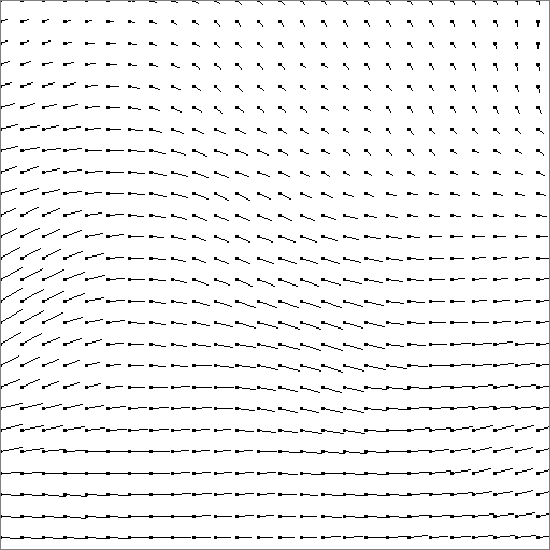
\includegraphics[width=0.5\textwidth]{imgs/eulerian.png}
    \label{fig:eulerian}
  }
  \subfloat[Lagrangian]{
    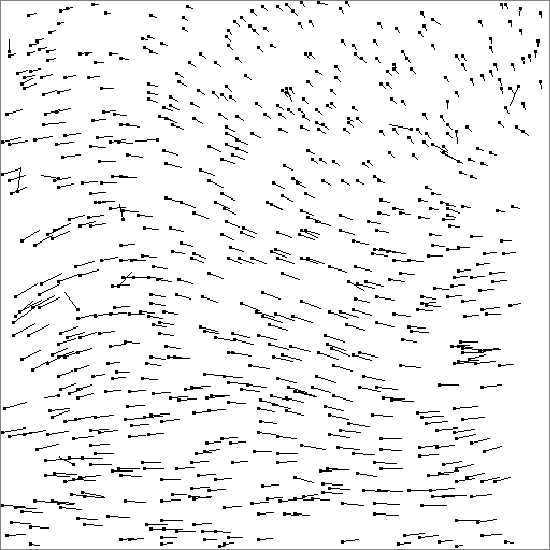
\includegraphics[width=0.5\textwidth]{imgs/lagrangian.png}
    \label{fig:lagrangian}
  }
  \caption{The eulerian and the lagrangian viewpoints.}
  \label{fig:eulerian-lagrangian}
\end{figure}

In the lagrangian viewpoint we let the measuring devices move along
the current in the fluid and take measurements at different locations
in the fluid. Here we imagen that the measuring device is part of the
fuild or a particle that the fluid moves around. Figure
\ref{fig:lagrangian} shows how the current has moved the devices as
time has progressed.

These two viewpoints are tightly coupled to the way the simulation data
is represented and visuliazed. Lets say that we are interested in
visualizing the surface of the substance.
%
The Lagrangian data is keept as points in space and moved around by
updating the position of the points. This can be visualizes by
imposing that the points define a surface and rendered as geometry
e.g. triangles between the points.
%
The eulerian viewpoint is seen as a 3D grid. Each cell in the grid has
a density that describes how much substance the cell contains (0-100\%).

Whiled this example focuses on measuring movement, the two different
viewpoints can be imposed on all kinds measurements.
%
When modelling a fluid, the Eulerian viewpoint is often
enough. But for more advanced simulations of fluid or solid,
Lagrangian is often used so the underlaying math equations are simpler
to describe.

%And example of this is: When modelling ...

%The are algoritmens that converts between the two viewpoints: .. . And
%as such nothing prevents us from using both viewpoint when defining
%the mathematically models that drives the simulation. As can be seen
%from the conversion algorithms, this envolves a fair amount of
%math. So to make the models more readable, it is advised to model
%in one of the domains, and only when optimizing the formulaes for
%performance, introduce conversions.

%In all the mathematically models that are developed in this repor the
%Lagrangian viewpoint is will be used.

%ref: fluids book, michael bang figures,

% \subsection{Data models}
% In the different parts of the simulator we use two different data
% model which are coupled tightly the the two points of view just
% reviewed. The two data models are refered to as the vertex/primitive
% model and the volumetric model. Each of which will now be elaborated.

% \subsubsection{The Vertex/Primitive model}
% When using the Lagragian viewpoint, we call the data model for a
% vertex/primitive model. In this model we have a vertex pool
% constituting which points are available, and some primitives, which
% referes to the vertices and binds these togther.

% \textbf{Primitives}
%  Fx as triangle, quads or tetrahedras.

% \subsubsection{The volumetric model}
% When using the Euler viewpoint in 2D, vi call the grid a texture and
% the cell for pixels. As we moves to 3D pixels are called voxels as
% they cover a volume.

% \textbf{density field}
% The voxels has value from 0 to 1. Which is to be interpreted as the
% procentage of solid the voxel contains.
% \textbf{Vector fields} \url{http://en.wikipedia.org/wiki/Vector_field}
% \textbf{Tensor fields} \url{http://en.wikipedia.org/wiki/Tensor_field}
% \textbf{energi density field}
% \url{http://users.powernet.co.uk/bearsoft/Field.html}

% \textbf{ISO Surface (level sets)}
% Each voxel is set to zero when it contains the surface of the solid
% and 1 all other places. \url{http://en.wikipedia.org/wiki/Isosurface}

% \textbf{distance field}
% Nearly the same as an iso surface. That is it zero on the surface, but
% instead of being 1 elseware, the voxels contains a value corresponding
% to the shortests distance to the surface.

% \textbf{signed distance field (SDF)}
% A distance field, but with a sign determining if the voxel is inside or
% outside the solid. So fx the distances inside the solid could be
% negative, and the voxels outside could be positive.

% The density field can be converted into a signed distance field or iso
% surface and rendered using standard volume rendering techniques.

% \subsubsection{Vertex/Primitive contra Volumetric}
% For a 3D graphics framework like OpenGL or DirectX, the
% vertex/primitive data model is the most convinient as data can be
% mapped directly to visual output.
% %
% But in some situations the vertex/primitive model is not the first
% choise. When representing the data as volumetric data the data model
% imposes a grid structure on the data, making some thing easier to
% do. Fx when doing collision detection the volumetric model has
% advantages.

% \subsection{Getting geometry input data}

% \subsubsection{X-ray images}
% The main source of surface and body (geometry) data comes from 3D X-ray
% image scans. X-ray images are volumetric data in black and white where
% each voxel has a value which describes the density in that voxel.
% When taking an X-ray image of bones or teeth, X-ray pulses are
% shot through the body with radiographic film behind. The bones or
% teeth absorb the most photons by the photoelectric process, because
% they are more electron-dense. The X-rays that do not get absorbed turn
% the photographic film from white to black, leaving a white shadow of
% bones and teeth on the film.

% \subsubsection{Segmentation}
% Patients are scanned and the dentist or other personal prepare
% the X-ray images for simulation by segmenting out the tooth that is to
% be operated upon in the simulator. As an example the segmentation can
% be done in the software ITK-Snap as showen in figure
% \ref{fig:itk-snap}, in the figure the red tooth has been segmented by
% first applying an automatic segmentation algorithm and afterwards rofly
% adapted by hand. The tooth segmented with green, has only been
% automaticly segmented, which also shows as the segmentation flows into
% the tooth next to it.

% \begin{figure}[H]
%   \centering
%   \includegraphics[width=14cm]{./images/itk-snap.png}
%   \caption{Segmentation in ITK-Snap.}
%   \label{fig:itk-snap}
% \end{figure}

% After the segmentation has taken place, the 3D image is exported, into
% a unsigned byte density field where voxels in the model (maked as red
% in the figure) get value 255, and voxels outside the model are set to
% 0. A guide of how to use ITK-Snap is provide in appendix \ref{guide:itk-snap}.

% \section{The simulator parts}
% The full simulator is made up of several different part or sub
% simulators. Each of the sub simulators does different things, and must
% therefore be designed specifictly for the job they need to handle. As
% mentioned in the introduction, we have identified the following
% different sub simulators. Now is that time to specify what they do and
% how we think it can be done.

% \subsection{Cutting tissue}
% As in: Virtual Reality
% Heart\footnote{\url{http://www.systematic.dk/om+os/innovation}}. I
% vertex based model and tools like knife and tweezers.

% \begin{figure}[H]
%   \centering
%   \includegraphics[width=14cm]{./images/heart-sim.png}
%   \caption{Screenshot from: The Heart Simulator.}
%   \label{fig:heart-sim}
% \end{figure}

% Picture from: \url{http://www.jespermosegaard.dk/Projects}

% \url{http://www.alexandra.dk/nyhedsbrev/to/05/november05/status_cavi.htm}
% \url{http://www.cavi.dk/projects/surgical_simulation.php}
% \url{http://www.daimi.au.dk/~mosegard/medVisSim/}
% \url{http://cg.alexandra.dk/2009/04/30/simulation-of-congenital-heart-surgery/}
% \url{http://www.daimi.au.dk/~cfpc/projects/cadiovas/cadiovas_summary.htm}

% \subsection{Dividing into smaller pieces}
% This job, has two distinct sub simulators, one for drilling and on for
% breaking. It has been divide this way, as the drilling is easiest done
% on a volumetric data model while the breaking is done using linear
% elastic model which are based on deforming the body making a vertex
% model more preferable.

% \subsubsection{Drilling}
% As the tooth have been segmented and exported from itk-snap, this data
% can be used directly in this sub simultor.
% %
% Drillng as done in the The Visible Ear
% Simulator\footnote{\url{http://www.alexandra.dk/ves/}}, are done
% directly on volumetric data. It works by simulating the drill head as
% a sphere, and when rotation the simulator modifies the voxels by
% removing material where the sphere are located.

% A possibility is to base the hardness of the material on the intensities
% of the material from the X-ray images.

% \begin{figure}[H]
%   \centering
%   \includegraphics[width=14cm]{./images/ear-sim.png}
%   \caption{Screenshot from: The Visible Ear Simulator.}
%   \label{fig:ear-sim}
% \end{figure}

% Picture taken from:
% \url{http://cg.alexandra.dk/category/visible-ear-simulator/}.

% To visualize the data, standard volumetric rendering techniques like
% ray tracing \ref{ray_tracing} or photon mapping \ref{photon_mapping}
% can be imployed. This is also what is done in The Visivle Ear
% Simulator.

% As all these techniques are implemented and used in The Visible Ear
% Simulator we can say for surtant that this is possible to simulate in
% real-time. But it is only possible because we do not need voxel models
% of the same magnitude as used in the ears simulator.

% \subsubsection{Breaking the tooth}
% As this sub simulator is the main topic of the thesis, it will be
% fulle described in the rest of the thesis. But to have an idear of
% what is to come this sub simulator models the tooth as a stiff
% material and tools for breaking the tooth are provided to the
% user. The model of the tooth uses triangles to model the surface
% and tetrahedrons for the body. We use the physics based elasticity
% theory and the finite element method to model deformation and
% energi. Lastly we employ fracture mechanics to model fracturing of the
% tooth when the energi raises above a limit defined for the material.

% \subsection{Removing pieces}
% This sub simulation is the least demanding simulation as all models
% in the sceen can be treated as ridig bodys, that is they cannot
% undergo deformation or other forms of modifications. They can only be
% move and rotated. So that main thing in this simulator is collision
% detection, which can be done naive on the GPU in real-time. The
% collision detection and tools needed here are very simulare to what is
% used in the heart simulation, and we are positive that this sub
% simulator will not be a problem to implement.

% \subsection{Stitching tissue}
% todo...

% \section{Binding the sub simulators together}
% Because the different sub simulator use different data models, we need
% to have a way of converting between the data models

% \subsection{Converting from Vertex/Primitive to Volumetric data}
% This convertion can be done by a algorithm known as flood filling.
% But to be able to use this algorithm the input model needs to be
% waterproof, meaning that the geometry must define a complete surface
% without any holes. A guide of how to do this convertion is provide in
% appendix \ref{guide:floodfilling}.

% \textbf{Generating Signed Distance Fields From Triangle Meshes}
% \url{http://citeseerx.ist.psu.edu/viewdoc/download?doi=10.1.1.111.6331&rep=rep1&type=pdf}

% \subsection{Converting from Volumetric to Vertex/Primitive data}
% This convertion can be done by a algorithm known as iso stuffing. ISO
% surface stuffing take a ISO surface as input, so to convert our
% density field we need to convert it to a ISO surface. A guide of how
% to do the density field to ISO surface converting and doing the ISO
% surface stuffing is provide in appendix \ref{guide:isosurfacestuffing}.

% \section{Hardware setup}
% Computer with monitor for visualisation, and some kind og haptic
% device for interacting with the simulator.

% \subsection{Haptic feedback}

% \begin{figure}[H]
%   \centering
%   \includegraphics[width=14cm]{./images/haptic_feedback.png}
%   \caption{Haptic feedback.}
%   \label{fig:haptic-feedback}
% \end{figure}

% \url{http://www.hjerteforeningen.dk/sw69890.asp}

%%% Local Variables: 
%%% mode: latex
%%% mode: auto-fill
%%% TeX-PDF-mode: t
%%% TeX-master: "../master.tex"
%%% End: 


\subsection{Sean}
The process of moving an implicit surface given by a signed distance function is known as \emph{level set methods}. Level set methods are ways of influencing signed distance fields to move the implicit surfaces contained therein. This is done by solving certain equations of motion that we will describe in this section.

As discussed previously\todoSean{Has it been mentioned before?}, using implicit surfaces rather than an explicit representation such as a polygon mesh provides certain benifits. Nowhere is this more clear than when implementing moving surfaces. Moving a surface built from triangles presents a number of problems. First and foremost, it becomes necessary to determine whether the surface starts to overlap itself and what to do if it does. Clearly this is problematic when dealing with polygons, since there is no obvious or "natural" way of merging two polygons which have overlapped.

\image{movingsurfaces.png}{0.4}{Two moving surface representations.
Top: Explicit representation, merging is a problem.
Bottom: Implicit surface by signed distance field, merging is automatic.}{velocity:movingsurfaces}

With implicit surfaces, this problem disappears, since an implicit surface is just that: implicit. If two "interior" areas of the implicit function "overlaps", it simply means that that area of the domain is in the interior of the function, and the interface will wrap around it as appropriate. See figure \vref{velocity:movingsurfaces} for an illustration of the advantage of implicit surfaces.

\subsection{The level set equation}
We examine now how to evolve an implicit surface, or interface, by affecting the underlying implicit function with an externally generated velocity field. This process of convection/advection \todoSean{One of these? Both?}is defined by equation \vref{velocity:levelseteq}
\begin{eqnarray}
\label{velocity:levelseteq}
\phi_t + \vec{V}\cdot \nabla \phi = 0
\end{eqnarray}
This simple convection equation is referred to as the \emph{level set equation} due to its central importance to level set methods. It describes the evolution of an implicit function $\phi$ by a velocity field $\vec{V}$. $\nabla \phi$, of course, is the gradient of the function. From this, we have
\begin{eqnarray}
\label{velocity:gradient}
\vec{V}\cdot\nabla\phi = u\phi_x + v\phi_y
\end{eqnarray}
Where $phi_x$ and $phi_y$ are the spacial derivatives in the first two dimensions respectively and $u$ and $v$ are the two components of the velocity vector.

Since we are essentially only interested in moving the implicit surface or interface with the velocity field, it is sufficient for the field to contain values only in a band around the interface. For simplicity of implementation, however, we assume that the field is defined across the entire domain.

For concrete implementation purposes, to evolve an implicit surface in an n-dimensional domain, the velocity field is an n-dimensional cartesian grid of n-dimensional vectors. In our two-dimensional case, that means all velocity fields are double arrays of two-value vectors.

\subsection{Upwind differencing}
How then, do we numerically solve equation \ref{velocity:levelseteq}? As we know, the implicit function is discretized into a cartesian grid of cells with $\Delta x$ representing the width and height of these cells in the theoretical continuous field. In our case this is a discretized signed distance field, each cell in the grid being of course a number representing the distance from the zero-isocountour. So too is the velocity field represented discretely with vectors, as mentioned previously.

Now, since motion takes place across time, we will need discretize our motion across time as well. We discretize time into steps of $\Delta t$. The n'th time step we denote $t^n$ and the state of the cartesian grid of our signed distance field at that time as $\phi^n$. Since the velocity also may change over time, this too is separated into discrete steps $\vec{V}$.

One way of discretizing equation \ref{velocity:levelseteq} is the simple \emph{forward Euler} method. Equation \vref{velocity:forwardeuler} shows how the time-dependant term $\phi_t$ of equation \ref{velocity:levelseteq} is discretized by forward Euler. 
\begin{eqnarray}
\label{velocity:forwardeuler}
\frac{\phi^{n+1}-\phi^n}{\Delta t}+\vec{V}^n\cdot\nabla\phi^n = 0
\end{eqnarray}
This is a first-order accurate method for time discretization, which \cit{osher2002level} suggests is adequate, based on practical experience.
Expanding the gradient as in \vref{velocity:gradient} we get
\begin{eqnarray}
\label{velocity:forwardeuler}
\frac{\phi^{n+1}-\phi^n}{\Delta t}+u\phi_{x}^n + v\phi_{y}^n = 0
\end{eqnarray}
To calculate this equation, then, we must find the spatial derivatives in the x and y directions. For this we can again use a first-order difference method. However, we need to pick a direction in which to calculate the derivative. That is, do we use
\begin{eqnarray}
D^+\phi &\approx & \frac{\phi_{i+1} - \phi_i}{\Delta x} \texttt{ or}\\
D^-\phi &\approx & \frac{\phi_i - \phi_{i-1}}{\Delta x}
\end{eqnarray}
These being forward and backwards difference, respectively. Naturally, we choose by examining the velocities given for the cell in question in the velocity field and take the difference in the direction of change. Not surprisingly, the term "Upwind differencing" is derived from this way of sampling in the direction of change. 
Although it might seem natural to simply use a central difference, according to \cit{osher2002level}, this is unstable with forward Euler time discretization.

The method, then, for each cell in the grid of the implicit function is as follows:
\begin{itemize}
\item Look up the velocity in the corresponding cell in the velocity field.
\item Calculate the appropriate forward/backwards difference
\item From these, arrive at the partial spatial derivative
\item Store the new cell value
\end{itemize}
When this has been done for the entire grid, overwrite it with the new values.
Essentially, we are "collecting" the values that need to be written to the current cell of the grid in the direction they come from via the velocity grid.

To ensure stability of this method, \cit{osher2002level} recommends limiting the time-step according to the \emph{Courant-Friedrich-Lewy} condition (CFL for short) which can be written as
\begin{eqnarray}
\Delta t < \frac{\Delta x}{\max \left\lbrace \left| u \right| \right\rbrace}
\end{eqnarray}
By enforcing this, we increase the guarantee that small errors are not amplified over time. The effects of an unstable method are commonly referred to as "exploding", for obvious reasons.

Finally, \cit{osher2002level} recommends methods such as an essentially nonoscillatory (ENO) way of computing more accurate spatial differences and total variation diminishing (TVD) Runge-Kutta for further accuracy in temporal difference. In short, ENO is a polynomial forward or backward difference function and Runge-Kutta is essentially a multiple-step version of the simpler forward Euler method we use.


%%% Local Variables: 
%%% mode: latex
%%% mode: auto-fill
%%% TeX-PDF-mode: t
%%% TeX-master: "../master.tex"
%%% End: 



\section{Motion (grow/shrink, mean-curvature, morph, CFG condition)}


In contract to section \vref{sec:extVel}, this section describes
motion using a internally generated velocity field.

\newpage

\subsection{Grow/Shrink}

\todoPtx{Grow/shrink!}

%%% Local Variables: 
%%% mode: latex
%%% TeX-master: "../../master"
%%% End: 

% Copy this code to grow.tex later?

One of the most simple things we can do, is to move the interface in
the normal direction $\vec{N}$ using a constant $a$, efficiently
scaling the iso-surface.

From equation \vref{velocity:levelseteq} we have:
\begin{equation}
  \phi_t + \vec{V}\cdot \nabla \phi = 0
\end{equation}
Since $a\vec{N}$ have the same direction as $\nabla{\phi}$, we have the following:
\begin{align*}
  a\vec{N}\cdot\nabla\phi &=
  a\frac{\nabla\phi}{|\nabla\phi|}\cdot\nabla\phi \\
  &= a\frac{|\nabla\phi|^2}{|\nabla\phi|} 
  = a|\nabla\phi|
\end{align*}

With corresponds to this level set equation:

\begin{equation}
  \phi_t + a |\nabla \phi| = 0
\end{equation}

\todoPtx{When $\phi$ is a signed distance function, something, something....}

\todoPtx{Write about this code}
\begin{lstlisting}
for(unsigned int x=0; x<width; x++) {
    for(unsigned int y=0; y<height; y++) {
        phi(x,y) += -a;
    }
}
\end{lstlisting}

\subsection{Mean-Curvature}

\todoPtx{Mean-Curvature}

%%% Local Variables: 
%%% mode: latex
%%% TeX-master: "../../master"
%%% End: 

\subsection{Morph}

\todoPtx{Morph}

%%% Local Variables: 
%%% mode: latex
%%% TeX-master: "../../master"
%%% End: 

\subsection{CFG condition (Stability)}

\todoPtx{CFG}

%%% Local Variables: 
%%% mode: latex
%%% TeX-master: "../../master"
%%% End: 



%%% Local Variables: 
%%% mode: latex
%%% mode: auto-fill
%%% TeX-PDF-mode: t
%%% TeX-master: "../master.tex"
%%% End: 


\chapter{Extensions}
\label{chap:extensions}

\section{Narrow-band}
\label{sec:narrowband}
\todoVester{skriv om narrow band}

\section{3D}
\label{sec:3d}

\section{CUDA}
\label{sec:cuda}

Improving the performance of our algorithms can be done in many ways,
but one of the more obvious ones are using parallel computing!

Currently, the most accessible way to run programs in parallel is
using the graphics computation unit (GPU). Modern GPUs are very
powerful, and major manufactures have released software development
kits (SDK) for utilise the GPU for general purpose computation.

One of these SDKs is nVidias CUDA\cit{cuda}. The only thing needed to
use CUDA is a nvidia graphics card that is relatively new (a few years
tops), and the free SDK found at the CUDA website.

As GPUs were developed to render graphics, they are optimized to work
on spatially coherent data. This makes many of our algorithms a
natural target, as we often only need information about neighbouring
data points.

% section?
\subsection{Memory?}

When a algorithm have been implemented using CUDA, there are many ways
to optimize it. Often memory access is the biggest problem.

Because of the architecture of GPUs, CUDA have many different types of
memory. Each with different properties and uses.

\todoPtx{Skriv om threads?}

% code

\begin{lstlisting}
#define GetPhi(phi,x,y,w) phi[x+w*(y)]

void cu_Init() {}


__global__ void reinit(float *phi,float* phi0, float* phin, 
                       unsigned int width, unsigned int height) {
    uint x = __umul24(blockIdx.x, blockDim.x) + threadIdx.x;
    uint y = __umul24(blockIdx.y, blockDim.y) + threadIdx.y;

    if (x > width || y > height)
        return;
    
    float xy = GetPhi(phi,x,y,width);

    float phiXPlus = 0.0f;
    float phiXMinus = 0.0f;
    float phiYPlus = 0.0f;
    float phiYMinus = 0.0f;        	
    if (x != width-1) phiXPlus  = (GetPhi(phi,x+1, y,width) - xy);
    if (x != 0)       phiXMinus = (xy - GetPhi(phi,x-1, y,width));
    
    if (y !=height-1) phiYPlus  = (GetPhi(phi,x, y+1,width) - xy);
    if (y != 0)       phiYMinus = (xy - GetPhi(phi,x, y-1,width));

    /* GetPhi(phin,x,y,width) = phiYPlus; */
    /* return; */


    float dXSquared = 0;
    float dYSquared = 0;
    float a = GetPhi(phi0,x,y,width);
    if (a > 0) {
        // formula 6.3 page 58
        float _max = max(phiXMinus, 0.0f);
        float _min = min(phiXPlus, 0.0f);
        dXSquared = max(_max*_max, _min*_min);
                    
        _max = max(phiYMinus, 0.0f);
        _min = min(phiYPlus, 0.0f);
        dYSquared = max(_max*_max, _min*_min);
    } else {
        // formula 6.4 page 58
        float _max = max(phiXPlus, 0.0f);
        float _min = min(phiXMinus, 0.0f);
        dXSquared = max(_max*_max, _min*_min);
                    
        _max = max(phiYPlus, 0.0f);
        _min = min(phiYMinus, 0.0f);
        dYSquared = max(_max*_max, _min*_min);        				
    }

    float normSquared = dXSquared + dYSquared;           
    float norm = sqrt(normSquared);

    // Using the S(phi) sign formula 7.6 on page 67
    //float sign = phi(x,y) / sqrt(phi(x,y)*phi(x,y) + normSquared);
    float sign = GetPhi(phi0,x,y,width) / 
        sqrt(GetPhi(phi0,x,y,width)*GetPhi(phi0,x,y,width) + 1);
    float t = 0.3; // A stabil CFL condition
    GetPhi(phin,x,y,width) = GetPhi(phi,x,y,width) - sign*(norm - 1)*t;


}

void cu_Reinit(float* data, 
               unsigned int w,
               unsigned int h,
               unsigned int iterations) {
    float* phiData;
    float* phi0Data;
    float* phinData;

    cudaMalloc((void**)&phiData, sizeof(float)*w*h);
    cudaMalloc((void**)&phi0Data, sizeof(float)*w*h);
    cudaMalloc((void**)&phinData, sizeof(float)*w*h);
    cudaMemcpy((void*)phiData,(void*)data, sizeof(float)*w*h,cudaMemcpyHostToDevice);
    cudaMemcpy((void*)phi0Data,(void*)data, sizeof(float)*w*h,cudaMemcpyHostToDevice);
    cudaMemcpy((void*)phinData,(void*)data, sizeof(float)*w*h,cudaMemcpyHostToDevice);


    CHECK_FOR_CUDA_ERROR();

    const dim3 blockSize(32,16,1);
    const dim3 gridSize(w/blockSize.x, h/blockSize.y);

    for (unsigned int i=0;i<iterations;i++) {
        reinit<<<gridSize,blockSize>>>(phiData,phi0Data,phinData,w,h);
        float* tmp = phiData;
        phiData = phinData;
        phinData = tmp;

        cudaThreadSynchronize();
        CHECK_FOR_CUDA_ERROR();
    }

    cudaMemcpy((void*)data,(void*)phiData, sizeof(float)*w*h,cudaMemcpyDeviceToHost);
    CHECK_FOR_CUDA_ERROR();
    cudaFree(phiData);
    cudaFree(phi0Data);
    cudaFree(phinData);
}

\end{lstlisting}

\todoPtx{CUDA coda}
\subsection{Results}

The results in table \ref{tbl:cudaRes} are taken from a system with a
1.8 Ghz Intel Core 2 Duo CPU, 4 GB RAM and a 512MB nVidia GeForce
9600M GT. The time is an average of about 100 iterations of the
algorithm.

\begin{table}[h]
  \centering
  \begin{tabular}{|l|r|r|r|}
    \hline    Algorithm & CPU & GPU & Speedup \\
    % BEGIN RECEIVE ORGTBL numbers
\hline
Reinitialization & 417825 usec & 136675 usec & 2.5987123 \\
- with textures & - & 100006 usec & 3.5515769 \\
\hline
    % END RECEIVE ORGTBL numbers
  \end{tabular}
  \caption{GPU vs. CPU comparison}
  \label{tbl:cudaRes}
\end{table}

The results shows a significant speedup. Using a quite
naive implementation the speedup is easily more than doubled on a inexpensive
consumer graphics card.

\todoPtx{Picture!}


% grep Reinit run1.log | grep CUDA | awk '{sum+=$7} END {print "avg=",sum/NR}'


\begin{comment}
#+ORGTBL: SEND numbers orgtbl-to-latex :splice t :skip 2
|------------------+-------------+-------------+-----------|
|                  | CPU         | GPU         |   Speedup |
|------------------+-------------+-------------+-----------|
| Reinitialization | 417825 usec | 136675 usec | 3.0570697 |
| - with textures  | -           | 100006 usec | 4.1779993 |
|------------------+-------------+-------------+-----------|
#+TBLFM: @2$4=@2$2 / @2$3::@3$4=@2$2 / @3$3
\end{comment}


%%% Local Variables: 
%%% mode: latex
%%% mode: auto-fill
%%% mode: orgtbl
%%% TeX-PDF-mode: t
%%% TeX-master: "../master.tex"
%%% End: 


\section{Segmentation}
\label{sec:segmentation}
\begin{comment}
  Martin har tænkt sig at skrive noget fornuftigt om segementering engang!
\end{comment}


\section{Fluid / Smoke}
\label{sec:fluid}

\section{Image reconstruction}
\label{sec:imagereconstruction}

\appendix

\newpage


\bibliographystyle{alpha}
\bibliography{text/levelset}


\end{document}


%%% Local Variables: 
%%% mode: latex
%%% mode: auto-fill
%%% TeX-PDF-mode: t
%%% TeX-master: t
%%% End: 
